%
% chapter.tex -- Kapitel 3: 1-Formen und Kurvenintegrale
%
% (c) 2024 Prof Dr Andreas Müller
%
\chapter{Differentialformen und Kurvenintegrale
\label{chapter:kurvenintegral}}
\kopflinks{Differentialformen und Kurvenintegrale}
Ein Flug zum Mars muss Energie aufwenden, um gegen die Schwerkraft der
Sonne von der Erdbahn aus zu der 
Entfernung von der Sonne zu gewinnen.
In der Praxis wird dies dadurch erreicht, dass man dem Raumfahrzeug
mithilfe von Raketentriebwerken genügend kinetische Energie erteilt.
Es folgt dann einer elliptischen Bahn, die ihren sonnenfernsten Punkt
bei der Marsbahn hat.
Während des Fluges wird laufend kinetische Energie des Raumschiffs in
potenzielle Energie umgewandelt werden.
Mit jedem kleinen Teilstück der Flugbahn verliert das Raumschiff 
kinetische Energie, die proportional ist zur Kraftkomponente parallel
zur Flugbahn. 
Das potentielle Energiepaket das während des Teilstücks gewonnen wird,
ist linear vom Tangentialvektor der Bahn abhängig.
Die gesamte potentielle Energie, die zwischen Erde und Marsbahn
gewonnen wird, ist die Summe dieser Teilstücke.
Mathematisch wird es durch eine Art Integral einer Funktion dargestellt,
welches sowohl linear von der Bahntangente wie auch vom Pfad des
Raumschiffs abhängt.
Diese Integralkonstruktion muss aber so erfolgen, dass Sie nicht von der
Wahl von Koordinatensystemen und Parametrisierungen abhängt, was in
diesem Kapitel durchgeführt werden soll.
Sie muss ausserdem so funktionieren, dass sie sich über mehrer
Koordinatensysteme hinweg zusammensetzen lässt, wie dies bei einer
Bahn auf einer Mannifaltigkeit unvermeidlich wird.

%
% 1-Formen
%
\section{1-Formen}
Was ist es eigentlich, was man integrieren will?
Zunächst gibt der riemannsche Integralbegriff aus dem elementaren
Analysisunterricht den Eindruck, dass es eine Funktion ist.
Es können aber nicht allein die Funktionswerte sein, die das Integral
bestimmen.
Vielmehr kommt es auch darauf an, wie ``schnell'' der Definitionsbereich
beim Integrieren durchlaufen wird.
Dies wird zum Beispiel durch die Substitutionsformel für das Integral
wiedergegeben.
Man kann sie auch als eine Koordinatenänderungsformel für das Integral
entlang der reellen Achse betrachten.
Was ist dann aber die koordinatenunabhängige Grösse, deren Integral
bestimmt worden ist?
Dies soll in diesem Abschnitt geklärt werden.

%
% Riemann-Integral
%
\subsection{Riemann-Integral}
Im elementaren Analysis-Unterricht lernt man, dass das Riemann-Integral
\[
I
=
\int_a^b f(x)\,dx
\]
einer Funktion $f(x)$ die Fläche unter der Kurve $y=f(x)$ berechnet.
Man macht das, indem man die Fläche in zunächst in vertikale Streifen
der Breite $\Delta x_i$ zerlegt, die an bei den Koordinaten $x_i$
beginnen.
Die Rechtecke dürfen sich nicht überlappen und müssen die Fläche unter
der Kurve vollständig abdecken, die Teilstellen $x_i$ müssen
also $x_{i+1}=x_i+\Delta x_i$ erfüllen.
Dann ist die Summe
\begin{equation}
\sum_{i} f(x_i)\cdot \Delta x_i
\approx 
I
\label{buch:kurvenintegral:1-form:eqn:riemann-summe}
\end{equation}
eine Approximation für den Wert des Riemann-Integrals.

Der Unterschied zum exakten Wert kommt vor allem daher, dass die
Rechtecke mit Breite $\Delta x_i$ und Höhe $f(x_i)$ manchmal
die Funktionskurve überragen, zum Beispiel wenn die Kurve negative
Steigung hat, und manchmal darunter bleiben, wenn die Kurve positive
Steigung hat.
Der Unterschied setzt sich aus Dreiecken zusammen, deren Grundseite
$\Delta x_i$ ist, und deren Höhe durch $f'(x_i)\cdot \Delta x_i$
beschränkt ist.
Der Fehler ist daher grössenordnungsmässig nicht grösser als
\[
\Delta I
\approx
\sum_i \Delta x_i \cdot |f'(x_i)\cdot \Delta x_i|
=
\sum_i |f'(x_i)| \Delta x_i^2.
\]
Sorgt man dafür, dass die Schritte $\Delta x_i$ alle gleich klein
sind, also $\Delta x_i=h$, dann folgt
\[
\Delta I
\approx
\sum_i |f'(x_i)| h^2
=
h\sum_i |f'(x_i)|h
\approx
h\int_a^b |f'(x)|\,dx.
\]
Für eine stetig differenzierbare Funktion ist $f'(x)$ im Integranden
auf der rechten Seite beschränkt.
Das Integral auf der rechten Seite ist also beschränkt.
Es bleibt aber der Faktor $h$, der den Fehler $\Delta I$ beliebig
klein macht, wenn man $h$ gegen $0$ gehen lässt.

%
% Substitution
%
\subsection{Substitution}
Der Integrand $f(x)$ im Riemann-Integral ist offenbar eine von
der Parametrisierung unabhängige Grösse.
Wechselt man die Koordinaten mit Hilfe einer Koordinatentransformation
$x(y)$, dann bleiben die Werte $f(x(y))$ an entsprechenden Stellen
des Definitionsbereiches die gleichen.
Es ändert sich aber das durch den Faktor $dx$ im Integral symbolisierte
Gewicht, mit dem jeder Summand in der Riemann-Summe
\eqref{buch:kurvenintegral:1-form:eqn:riemann-summe}
gewichtet wird.
Die Koordinatentransformation $x(y)$ macht aus einem Schritt $\Delta y$
einen $x$-Schritt von der Grössenordnung
\[
\Delta x
\approx
\frac{dx}{dy}(y)\cdot \Delta y.
\]
Sind $a'$ und $b'$ die Endpunkte des $y$-Intervalls, die auf 
$a=x(a')$ und $b=x(b')$ abgebildet werden, dann ist daher das
Integral
\begin{equation}
\int_a^b f(x)\,dx
=
\int_{a'}^{b'} f(x(y)) \, \frac{dx}{dy}(y)\,dy.
\label{buch:kurvenintegral:1-form:eqn:substitution}
\end{equation}
Dies ist die bekannt Formel für die Substitutionsformel für das Integral.


%
% Integral über ein eindimensionales Definitionsgebiet
%
\subsection{Integral über ein eindimensionales Definitionsgebiet}
%
% fig-1koordinaten.tex
%
% (c) 2025 Prof Dr Andreas Müller
%
\begin{figure}
\centering
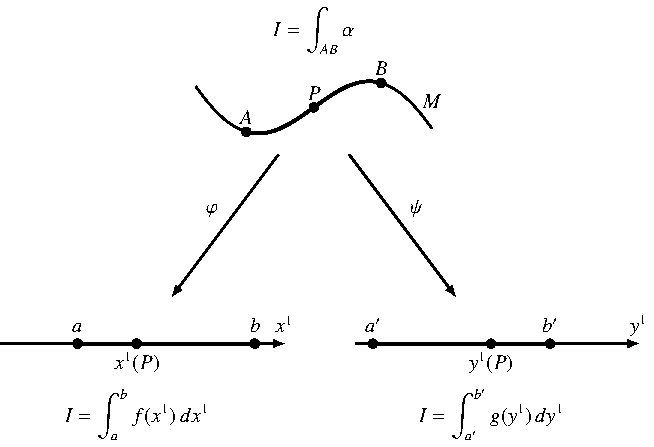
\includegraphics{chapters/030-kurvenintegral/images/1koordinaten.pdf}
\caption{Verschiedene Koordinatensysteme für ein eindimensionales
Definitionsgebiet $M$, auf dem ein Integral berechnet werden soll.
Oben steht ein koordinatensystemunabhängiges Konzept für eine Integral, 
welches in verschiedenen Koordinaten durch ein Riemannsches Integral
berechnet werden kann.
Die Substitutionsformel für das Integral liefert das
Koordinatentransformationsgesetzt zwischen den Darstellungen
$f(x^1)\,dx$ und $g(y^1)\,dy^1$ von $\alpha$.
\label{buch:kurvenintegral:fig:1koordinaten}}
\end{figure}

Die Substitutionsformel erklärt, wie das Integral angepasst werden
muss, wenn man von einer Koordinatenwahl $x$ zur alternativen
Koordinate $y$ wechseln will.
Wir können das Integral aber auch als eine Zahl betrachten,
die nur von zwei rein geometrisch definierten Eigenschaften
abhängig sind.
Einerseits ist dies eine Teilmenge eines eindimensionalen
Definitionsgebietes, welches in
Abbildung~\ref{buch:kurvenintegral:fig:1koordinaten} durch
den Bereich zwischen den Punkten $A$ und $B$ entlang der Menge $M$
symbolisiert ist.
Durch die Koordinatenssysteme $\varphi$ und $\psi$ werden daraus
die Intervalle $[a,b]$ von $x^1$-Koordinatenwerten bzw.~$[a',b']$
von $y^1$-Koordinatenwerten.

Die zweite Komponente zur Definition des Integrals ist eine
noch zu definierende Grösse $\alpha$, die die Funktionswerte
entlang des Definitionsgebietes liefert.
Dies muss so geschehen, dass $\alpha$ wieder ein Objekt ist,
welches vom Koordinatensystem unabhängig definiert ist, oder 
besser, dessen Transformationseigenschaften beim Koordinatenwechsel
klar sind.
Als Leitlinie für die gesuchte Umrechnungsformel kann die
Substitutionsformel
\eqref{buch:kurvenintegral:1-form:eqn:substitution}
herangezogen werden.

Das gesamte Integral möchten wir als
\[
\int_{AB} \alpha
\]
schreiben können.
Es soll die üblichen Eigenschaften eines Integrals haben, also
insbesondere linear sein:
\[
\int_{AB}
(\alpha + \beta)
=
\int_{AB}
\alpha
+
\int_{AB}
\beta
\qquad\text{und}\qquad
\int_{AB}
t
\alpha
=
t
\int_{AB}
\alpha.
\]
In einem Koordinatensystem soll eine Integralformel entstehen.
Rein formal ist daher $\alpha$ in den Koordinatensystemen $\varphi$
bzw.~$\psi$ durch
\[
f(x^1)\,dx^1
\qquad
\text{bzw.}
\qquad
g(y^1)\,dy^1
\]
gegeben.
Die Substitutionsformel
\eqref{buch:kurvenintegral:1-form:eqn:substitution}
besagt dann, dass
\[
g(y^1)
= 
f(\varphi\circ\psi^{-1}(y^1))
\frac{dx^1}{dy^1}(y^1)
=
f(\varphi\circ\psi^{-1}(y^1))
\frac{d}{dy^1}(\varphi\circ\psi^{-1}(y^1))
\]
sein muss.
Man beachte, dass $g(y^1)$ und $f(x^1)$ nicht Komponenten eines
Vektors sind, dann für Vektorkomponenten $v_1$ gilt wegen
\[
\frac{\partial}{\partial y^1}
=
\frac{dx^1}{\partial y^1}\cdot \frac{\partial }{\partial x^1}.
\]
die Umrechnungsformel
\[
v_1'(y^1)
=
\frac{dy^1}{dx^1}
v_1(x^1)
\qquad\text{oder}\qquad
v_1(x^1)
=
\frac{dx^1}{dy^1} v_1'(y^1).
\]
Die Transformation erfolgt also in der ``falschen'' Richtung.

Aus der Sicht des angestrebten Ziels, ein koordinatenunabhängiges
Integralkonzept zu definieren, ist die gegenüber Vektoren ``verkehrte''
Transformationsrichtung zu erwarten.
Wenn ein Koordinatenwechsel dazu führt, dass der Koordinatenraum
langsamer durchlaufen wird, äussert sich das darin, dass die Komponenten
eines Tangentialvektors grösser werden.
Der Tangentialvektor beschreibt aber die ``Schrittgrösse $dx$'' beim
Integrieren auf koordinatenunabhängige Art.
Damit das Integral gleich bleibt, muss der skalare Faktor entsprechend
kleiner werden.

%
% Transformation von Linearformen
%
\subsection{Linearformen}
Die im vorangegangenen Abschnitt heuristisch hergeleitete
Transformationseigenschaft ist nicht so überraschend, man kann sie
auch in der linearen Algebra bei Linearformen finden.
In diesem Abschnitt soll die Koordinatentransformationsregel für
Linearformen formuliert werden.

%
% Koeffizienten einer Linearform
%
\subsubsection{Koeffizienten einer Linearform}
Seien $a^i$ die Komponenten eines Vektors $a$ in einer Basis $e_i$ und
$t_{i}\mathstrut ^k$ die Koeffizienten der Transformationsmatris
in eine alternative Basis $e'_k$.
Die Komponenten in der alternativen Basis werden mit $a^{\prime k}$
bezeichnet und die Umrechung zwischen den Koordinaten erfolgt mit der
Formel
\begin{equation}
a^{\prime k}
=
t_i\mathstrut^k a^i
\label{buch:kurvenintegral:1formen:linearformen:vektor}
\end{equation}
gegeben.

Eine Linearform ist eine lineare Abbildung $l\colon V\to\mathbb{R}$,
die einem Vektor $v$ einen Zahlenwert $l(v)$ zuordnet.
Die Linearität verlangt, dass der Wert
\[
l(a)
=
\sum_i
l(a^ie_i)
=
a^i \underbrace{l(e_i)}_{\displaystyle=l_i}
\]
ist (man beachte die einsteinsche Summationskonvention).
Die Werte $l_i=l(e_i)$ sind die Koeffizienten, mit denen die $a^i$
multipliziert werden müssen, um $l(a)$ zu ergeben.
Entsprechend sind die $l'_i=l(e'_i)$ die Koeffizienten der Basis

%
% Transformation der Koeffizienten einer Linearform
%
\subsubsection{Transformation der Koeffizienten einer Linearform}
Bei der Koordinatentransformation soll sich der Wert $l(a)$ nicht
ändern, es muss daher
\[
l'_k
a'^k
=
l'_k
(t_i\mathstrut^k a^i)
=
(l'_kt_i\mathstrut^k) a^i
=
l_i
a^i
\]
sein.
Da dies für jeden beliebigen Vektor gelten muss, müssen die Koeffizienten
übereinstimmen und es folgt das Transformationsgesetz
\begin{equation}
l'_kt_i\mathstrut^k
=
l_i
\label{buch:kurvenintegral:1formen:linearformen:linearform}
\end{equation}
für die Koeffizienten der Linearform.
Die Transformation der Linearformkoeffizienten erfolgt also
in der umgekehrten Richtung vom gestrichenen Koordinatensystem 
zum ungestrichenen.
Ausserdem wird über den obneren Index von summiert statt über
den unteren wie in 
\eqref{buch:kurvenintegral:1formen:linearformen:vektor}.

Betrachtet man die Koeffizienten $t_i\mathstrut^k$ als Matrix, mit der
die Umrechnung der Koeffizienten von $a$ erfolgt, dann ist die Matrix,
mit der die Koeffizienten $l_k'$ umberechnet werden, die transponierte
Matrix.

%
% Kovariante und kontravariante Indizes
%
\subsubsection{Kovariante und kontravariante Indizes}
Die Koeffizienten einer Linearform und die Komponenten eines Vektors 
haben also entgegengesetztes Transformationsverhalten.
Es können die gleichen Koeffizienten der Transformationsmatrix 
verwendet werden, aber die Transformation erfolgt in der umgekehrten
Richtung und es muss über den anderen Index summiert werden.
Das unterschiedliche Verhalten wurde bereits durch die unterschiedliche
Position der Indizes vorweggenommen.
Während Vektorkomponenten obere Indizes verwenden, haben die
Koeffizienten einer Linearform untere Indizes.

\begin{definition}[kovariant und kontravariant]
Die Komponenten eines Vektors heissen {\em kontravariant}, sie haben
\index{kontravariant}%
einen hochgestellten Index, der ebenfalls {\em kontravariant} genannt
wird.
Die Koeffizienten einer Linearform von Vektoren heissen dargegen
{\em kovariant}, sie tragen einen unteren Index, der entsprechend
\index{kovariant}%
{\em kovariant} genannt wird.
\end{definition}

%
% Tensoren
%
\subsubsection{Tensoren}
Wir werden später sehen, dass es sinnvoll sei kann, dass eine Grösse
mehr als einen Index haben kann.
Zum Beispiel hängt die Kraft auf eine bewegte Ladung linear von der
Richtung des Magnetfeldes und von der aktuellen Bewegungsrichtung ab.
Beide Einflussfaktoren haben vektoriellen Charakter, werden also durch
Komponenten beschrieben, die ihrerseits verschiedene Komponenten haben.
Daher vereinheitlichen und verallgemeinern wir die Konzepte von Vektoren
und Linearformen zum neuen Begriff des Tensors.

Als etwas konkreteres Beispiel betrachten wir das Skalarprodukt von
zwei Vektoren $u$ und $v$ mit den Komponenten $u^i$ bzw.~$v^k$.
In der Vektorgeometrie lernt man, dass man das Skalarprodukt mit der
Formel $\sum_i u^iv^i$ berechnen kann.
Man lernt aber auch, dass diese einfache Formel nur für in einem
orthonormierten Koordinatensystem gilt, wo die Basisvektoren
orthogonal sind und Länge $1$ haben.
Insbesondere ist die angegebene Formel für das Skalarprodukt nicht
für beliebige Koordinatensysteme tauglich.

Schreibt man die Vektoren $u$ und $v$ explizit als Linearkombinationen
\[
u = \sum_{i=1}^n u^i b_i
\qquad\text{und}\qquad
v = \sum_{k=1}^n v^k b_k
\]
der Basisvektoren, dann ist das Skalarprodukt durch
\[
u\cdot v
=
\sum_{i,k=1}^n u^iv^k \underbrace{(b_i\cdot b_k)}_{\displaystyle g_{ik}}
\]
gegeben.
Für eine orthonormierte Basis sind die Koeffizienten
\[
g_{ik}
=
\left\{
\begin{array}{llcl}
1&\quad i=k&\qquad\Leftrightarrow\qquad&\text{Basisvektor $b_i$ hat Länge $|b_i|=1$}\\
0&\quad i\ne k&\qquad\Leftrightarrow\qquad&\text{Basisvektoren $b_i$ und $b_k$ sind orthogonal: $b_i\perp b_k$}
\end{array}
\right.
\]
Für beliebige Koordinatensysteme muss aber zugelassen werden, dass 
die Koeffizienten $g_{ik}$ beliebige Werte annehmen können.

\begin{definition}[metrischer Tensor]
Die Koeffizienten $g_{ik}$, die das Skalarprodukt zweier Vektoren durch
\[
u\cdot v
=
\sum_{i,k=1}^n u^iv^k g_{ik}
\]
heisst der {\em metrische Tensor}.
\index{metrischer Tensor}%
\end{definition}

Der metrische Tensor hat interessante zusätzliche Eigenschaften.
Er ist zum Beispiel symmetrisch, was sich in $g_{ik}=g_{ki}$ für
alle Paare $i,k$ äussert.
Ausserdem ist das Skalarprodukt üblicherweise positiv definit,
so dass 
\[
g_{ik}u^i u^k
>
0
\]
für von $0$ verschiedene Vektoren $u$ gilt.

Der metrische Tensor definiert das Skalarprodukt, welches eine bilineare
Abbildung ist, die aus zwei Vektoren auf jeweils lineare Art einen
Zahlenwert berechnet.
Man kann ihn aber auch anders interpretieren.
Gibt man nur einen Vektor mit den Komponenten $v^i$ vor, erzeugt der
metrische Tensor eine Linearform mit den Koeffizienten
\[
l_k = g_{ki}v^i
\]
Die Komponenten $l_k$ kann man auch ermitteln, indem man das Skalar
von $v$ mit den Basisvektoren berechnet.
Man kann also die Indizes des metrischen Tensors als Indizes betrachten,
die mit einem Inputvektor verknüpft werden, oder alternativ als Indizes
der Komponenten der Output-Linearform.

Es ist auch denkbar, anstelle von Vektoren aus Linearformen
neue Werte zu berechnen, oder mehr als zwei Faktoren einfliessen zu
lassen.
Zum Beispiel kann die Krümmung des Raumes dadurch beschrieben werden,
dass der Transport eines Vektors (erster Inputvektor) beim Paralleltransport
entlang eines Parallelogramms (zwei weitere Inputvektoren) gedreht wird.
Die Krümmung berechnet also auf lineare Weise aus drei Inputvektoren
einen Outputvektor.

\begin{definition}[Tensor]
\index{Tensor}
Ein {\em Tensor $r$-ter Stufe} ist eine multilineare Abbildung, die
$r$ Vektoren oder Linearformen auf Skalare abbildet.
Seine Komponenten sind durch eine Grösse
$A^{i_1\dots i_k}\mathstrut_{i_{k+1}\dots i_r}$
mit $r$ Indizes gegeben.
Der Tensor heisst vom Typ $(k,r-k)$ wenn er $k$ kovariante und 
$r-k$ kontravariante Indizes hat.
\end{definition}

Ein Skalar ist ein Tensor nullter Stufe.
Ein Vektor ist ein Tensor erster Stufe mit einem kontravarianten Index,
also vom Typ $(0,1)$, während eine Linearform ein Tensor erster
Stufe vom Type $(0,1)$ ist.
Der metrische Tensor $g_{ik}$ ist ein Tensor zweiter Stufe vom Typ
$(2,0)$.
Ein Tensor vom Typ $(1,1)$ hat Komponenten $a^i\mathstrut_k$, die aus
einem Vektor $u^k$ den Vektor mit den Komponenten
\[
v^i = a^i\mathstrut_k u^k
\]
berechnet.
Dies entspricht der Idee einer Matrix, die Vektoren auf andere 
Vektoren abbildet und die man in der linearen Algebra kennenlernt.

Beim metrischen Tensor sind die beiden Indizes wegen der Symmetrie
vertauschbar.
Man beachte aber, dass die Platzierung der Indizes im Allgemeinen nicht
beliebig ist.
Zum Beispiel wird der Riemannsche Krümmungstensor oft in der Form
\(
R^i\mathstrut_{klr}
\)
als Tensor vierter Stufe vom Typ $(3,0)$ geschrieben.
Er ist antisymmetrisch in den letzten beiden Indizes, es gilt also
\(
R^i\mathstrut_{klr}
=
-
R^i\mathstrut_{krl}
\),
es gibt aber keine offensichtlichen weiteren Symmetrien.
Wendet man den Tensor auf zwei Vektoren mit Komponenten $u^l$ und
$v^r$ an, erhält man
\[
a^i\mathstrut_k
=
R^i\mathstrut_{klr}u^lv^r,
\]
worin nur noch die zwei Indizes $i$ und $k$ frei sind.
Der Tensor $a^i\mathstrut_k$ zweiter Stufe vom Typ $(1,1)$
kann als eine Abbildungsmatrix betrachtet werden,
die einen Vektor auf einen anderen Vektoren abbildet.

Da die einsteinsche Summationskonvention nur über verschieden platzierte
Indizes summiert, wird sichergestellt, dass Linearformen nur auf
Vektorkomponenten angewendet werden können.
Da die Transformationsmatrix einen oberen und einen unteren Index hat,
kann sie aus einem kontravarianten Vektor nur wieder einen kontrvarianten
Vektor machen.
Ebenso wird ein kovarianter Index durch Transformation wieder zu einem
kovarianten Index.

%
% Tensoren sind nicht nur Matrizen mit mehr Dimensionen
%
\subsubsection{Tensoren sind nicht nur Matrizen mit mehr Dimensionen}
Auf den ersten Blick besteht eine grosse Ähnlichkeit zwischen dem
Konzept der Matrix und einem Tensor zweiter Stufe.
In der linearen Algebra schreibt man eine lineare Abbildung in einer
Basis durch eine Matrix.
Die Komponenten $u_k$ eines Vektors $u$ werden von der Matrix $A$
mit den Einträgen $a_{ik}$ durch
\[
v = Au
\qquad\Leftrightarrow\qquad
v_i = \sum_{k=1}^n a_{ik}u_k
\]
auf einen Vektor $v$ abgebildet.
Der erste Index, der Zeilenindex, bezeichnet die Komponente, die berechnet
wird, während über den zweiten Index summiert wird.
Ein Matrix wird meistens als rechteckiges Zahlenschema
\[
A
=
\begin{pmatrix}
a_{11} & a_{12} & \dots  & a_{1n} \\
a_{21} & a_{22} & \dots  & a_{2n} \\[-2pt]
\vdots & \vdots & \ddots & \vdots \\[-1pt]
a_{m1} & a_{m2} & \dots  & a_{mn}
\end{pmatrix}
\]
dargestellt.
Die Wirkung einer Matrix auf einem Vektor wird durch das Produkt
``Zeile mal Spalte'' gegeben, summiert wird immer über den zweiten
Index,, den Spaltenindex.

Tensoren erweitern diese Idee in mehrfacher Hinsicht.
Zunächst wird die Möglichkeit zusätzlicher Indizes geschaffen.
Man könnte die Koeffizienten als drei- oder noch höherdimensionales
Zahlenschema darstellen.
Allerdings ist dies auch nicht weiter hilfreich für die zweite
Erweiterung: jeder Index kann als Summationsindex verwendet werden.

In der Matrizenrechnung wird kein Unterschied zwischen kovarianten
und kontravarianten Indizes gemacht.
Es ist durchaus üblich, die Koeffizienten $g_{ik}$ des metrischen
Tensors als Einträge einer Matrix zu betrachten.
Sie wird die {\em Gram-Matrix} genannt und kann dazu verwendet
\index{Gram-Matrix}T
werden, das Skalarprodukt als 
\[
u\cdot v
=
u^t G v
=
\sum_{i,k=1}^n
g_{ik}u_iv_k
\]
zu schreiben.
Allerdings sind die Koeffizienten
\[
\sum_{k=1}^n a_{ik}u_k
\qquad\text{und}\qquad
\sum_{k=1}^n g_{ik}v_k
\]
für die Abbildungsmatrix bzw.~den metrischen Tensor von ganz verschiedenem
Charakter.
Im ersten Fall entstehen Komponenten eines Vektors, die sich bei Basiswechsel
kontravariant transformieren, im zweiten Fall entstehen Koeffizienten
einer Linearform, die sich kovariant transformieren.
Die bisherige Entwicklung hat aber gezeigt, dass diese Unterscheidung
wesentlich ist, wenn man dem Ziel einer koordinatenunabhängigen
Beschreibung von Naturgesetzen näher kommen will.

%
% Integrand $\alpha$ als Linearform
%
\subsubsection{Integrand $\alpha$ als Linearform}
Der Integrand eines koordinatenunabhängig definirten Integrals entlang
eines eindimensionalen Definitionsgebietes muss also eine
Linearform sind.
Tatsächlich wird das Arbeitsintegral in der Physik definiert als
das Wegintegral der Kraft entlang eines Weges definiert.
Darin wird die Kraft skalar mit dem Tangentialvektor multipliziert
und integriert.
Wir haben das Skalarprodukt bereits durch den metrischen Tensor
beschrieben.
Aus dem Kraftvektor mit den Komponenten $F^k$ macht er die Linearform
mit den Koeffizienten $g_{ik}F^i$.

Solche Linearformen werden auch als $1$-Formen bezeichnet.
Wir werden für Integranden über Gebiete höherer Dimension weitere

%
% Die Koordinaten-1-Formen
%
\subsection{Die Koordinaten-1-Formen}
Ein spezieller Fall tritt ein, wenn der Koeffizient der Integranden-1-Form
$\alpha$ die Zahl $1$ ist.
In diesem Koordinatensystem wird das Integral
\[
\int_{AB} \alpha
=
\int_{a}^{b} 1\, dx^1
=
\int_{a}^b\,dx^1
=
\bigl[ x^1 \bigr]_a^b
=
b-a.
\]
Im $y^1$-Koordinatensystem ist hat das Integral dagegen den Wert
\begin{equation}
\int_{AB}\alpha
=
\int_{a'}^{b'} \frac{dx^1}{dy^1}\,dy^1
=
\bigl[x^1(y^1)\bigr]_{a'}^{b'}
=
x^1(b') - x^1(a')
=
b-a,
\label{buch:kurvenintegral:1formen:eqn:hauptsatz}
\end{equation}
wobei im zweiten Schritt verwendet wurde, dass der Integrand die
Ableitung der Funktion $x^1(y^1)$ nach der Integrationsvariable ist.
Die Funktion $x^1(y^1)$ ist daher die
Stammfunktion des Integranden im zweiten Integral ist.
Wie erwartet, stimmen die Integrale überein.

Die Symbole $dx^1$ und $dy^1$ können daher genauso als Basislinearformen
betrachtet werden, wie die Ableitungsoperatoren
$\partial/\partial x^1$ und $\partial/\partial y^1$ als
Basisvektoren für die Tangentialvektoren betrachtet wurden.
Sie heissen die Koordinaten-1-Formen und sind besonders einfach
zu integrieren.

Eine $1$-Form $\alpha$ hat in einer Dimension die Form
\[
\alpha
=
f(x^1) \,dx^1
\]
und ihr Integral über das Intervall zwischen $A$ und $B$ ist
\[
\int_{AB}\alpha
=
\int_a^b f(x^1)\,dx^1.
\]
Die Notation ist so gewählt, dass sich die neue Betrachtungsweise als
Integral einer 1-Form über ein eindimensionales Gebiet nach Einführung
eines Koordinatensystems mit der konventionellen Riemann-Integration
deckt.

Das Resultat
\eqref{buch:kurvenintegral:fig:1koordinaten}
ist auch als der Hauptsatz der Infinitesimalrechnung bekannt.
Wir halten jedoch fest, dass es von einer Form ist, der wir später
wiederholt begegnen werden.
Das Integral der Ableitung einer Funktion über ein Intervall hat einen
Wert, der nur von den Werten der Funktion auf dem Rand des Intervalls
bestimmt ist.
Der Satz von Stokes wird später zeigen, dass dies ein allgemeines
Phänomen ist.
Das Integral einer geeignet definierten Ableitung eines Integranden
ist bestimmt durch die Werte auf dem Rand des Integrationsgebietes.
Dazu muss aber zunächst die Klasse der möglichen Integranden von
$1$-Formen auf $p$-Formen ausgweitet werden und es muss eine Ableitung
für $p$-Formen konstruiert werden.
Dies wird in den nachfolgenden Abschnitten und Kapiteln geschehen.

%
% Kurvenintegral einer 1-Form
%
\section{Kurvenintegral einer 1-Form}
Eine Kurve ist eine eindimensionale Untermannigfaltigkeit in
einer $n$-dimensionalen Mannigfaltigkeit $M$.
Eine $1$-Form auf der Mannigfaltigkeit $M$ führt zu einer 
$1$-Form auf der Kurve und damit wird es möglich, das Integral
dieser 1-Form auf der Kurve zu berechnen.
Dies soll in diesem Abschnitt schrittweise durchgeführt werden.

\subsection{$1$-Form auf einer Mannigfaltigkeit}
Eine $1$-Form auf einer $n$-dimensionalen Mannigfaltigkeit ist eine
Linearform, die auf einen Tangentialvektor angewendet werden kann
und einen Zahlenwert ergibt.
In einem Koordinatensystem mit den Koordinaten $x^1,\dots,x^n$ bilden
die Tangentialvektoren an die Koordinatenlinien eine Basis des
Tangentialraumes.
Die einzelnen Basisvektoren sind früher auch schon mit den
Ableitungsoperatoren $\partial/\partial x^i$ identifiziert worden.
Die Koordinaten-1-Formen $dx^1,\dots,dx^n$ ermitteln, wie schnell sich
die entsprechende Koordinate entlang eines Tangentialvektors ändert.
Da sich entlang einer Koordinatenlinie immer nur eine einzige
Koordinate ändert, gilt
\[
\biggl\langle dx^i,\frac{\partial}{\partial x^k}\biggr\rangle
=
\delta_{ik}
=
\begin{cases}
1&\qquad \text{falls $i=k$}\\
0&\qquad \text{sonst}.
\end{cases}
\]
Man nennt diese Basis der Linearformen auch die zur Basis der
Ableitungsoperatoren {\em duale Basis}.

Eine $1$-Form auf der Mannigfaltigkeit hat daher im Koordinatensystem
mit den Koordinaten $x^i$ die Form
\[
\alpha
=
\alpha_i(x)\, dx^i,
\]
wobei wieder die Summationskonvention gilt.

\begin{beispiel}
Die $1$-Form
\[
\beta
=
-
\frac{GMx^i}{r^3}
dx^i
\]
soll auf dem Impulsvektor eines Teilchens berechnet werden.
Wird die Bahnkurve mit der Zeit parametrisiert, hat der Geschwindigkeitsvektor
die Komponenten $\dot{x}^i$.
Der Impuls $p$ des Teilchens ist der Vektor mit den Komponenten
$p^i=m\dot{x}^i$.
Wendet man die Linearform $\beta$ darauf an, ergibt sich
\begin{align*}
\langle \alpha, p\rangle
&=
-
\frac{GMm}{r^3}
\biggl\langle \sum_i x^i\,dx^i, \sum_k\dot{x}^k\frac{\partial}{\partial x_k}\biggr\rangle
=
-
\frac{GMm}{r^3}
\sum_{i,k} x^i \biggl\langle dx^i,\dot{x}^k\frac{\partial}{\partial x_k}\biggr\rangle
\notag
\\
&=
-
\frac{GMm}{r^3}
\sum_{i,k}
x^i \delta_{ik} \dot{x}^k
=
-\frac{GMm}{r^3}
\sum_i x^i\dot{x}^i
\label{buch:kurvenintegral:kurvenintegral:eqn:gravimpuls}
\end{align*}
Dies ist die Leistung, die das Teilchen entgegen dem Gravitationsfeld 
arbeitet.
Eine $1$-Form ist also dazu geeignet, ein wichtiges physikalisches Konzept
des Gravitationsfeldes auszudrücken.

Die Form
\eqref{buch:kurvenintegral:kurvenintegral:eqn:gravimpuls}
ist allerdings noch nicht wirklich geeignet.
In der Formel wirden kontravariante Komponenten miteinander multipliziert
und summiert, dies führt nicht eine koordinatensystemunabhängige
Grösse.
Die Schwierigkeit rührt von der Darstellung des Impulses her, die später
noch modifiziert werden muss.
% XXX wo wird das geflickt?
\end{beispiel}

%
% Abbildung auf einer $1$-Form
%
\subsection{Abbildung einer $1$-Form}
Sei wieder eine $1$-Form $\alpha$ auf einer $n$-dimensionalen Mannigfaltigkeit
durch die Koeffizienten $\alpha_i(x)$ gegeben.
Sei ausserdem $f\colon N\to M$ eine differenzierbare Abbildung einer
$m$-dimensionalen Mannigfaltikgiet $N$.
Ein Tangentialvektor von $N$ im Punkt $p$ wird dargestellt durch eine
Kurve durch den Punkte $p$ in $N$.
Durch die Abbildung $f$ wird die Kurve auf eine Kurve durch den Bildpunkt
$q=f(p)$ abgebildet.
Da die Abbildung $f$ differenzierbar ist, entspricht der Bildkurve 
ein Tangentialvektor im Punkt $f(p)$.
Dies ist die tangentialabbildung $Tf\colon TN\to TM$, die Tangentialvektoren
von $N$ auf Tangentialvektoren von $M$ abbildet.

Eine $1$-Form berechnet aus einem Tangentialvektor einen Zahlenwert.
Die $1$-Form $\alpha$ auf $M$ tut dies für Tangentialvektoren $X$ von
$M$, nicht aber für Tangentialvektoren von $N$.
Dazu muss erst die Abbildung $Tf$ angewendet werden, die aus dem
Tangentialvektor $Y\in T_pN$ einen Tangentialvektor $T_pf(Y)=X\in T_qM$
macht.
Die Abbildung
\[
Y\mapsto \langle \alpha, T_pf(Y)\rangle \in \mathbb{R}
\]
ist eine lineare Abbildung, denn die Abbildung $T_pf$ ist linear und
Auswertung $X\mapsto \langle\alpha,X\rangle$ ist ebenfalls linear.
Die $1$-Form $\alpha$ auf $M$ definiert damit auch eine $1$-Form auf
$N$, die wir mit $T_pf^*\alpha$ bezeichnen.

\begin{beispiel}
Sei $N=\mathbb{R}$ eindimensional und $M=S^2$ eine Kugel.
Die Abbildung 
\begin{equation}
f
\colon
\mathbb{R}\to S^2
:
t
\mapsto 
\frac{1}{\cosh kt}
\begin{pmatrix}
\cos t\\
\sin t\\
\sinh kt
\end{pmatrix}
\label{buch:kurvenintegral:kurvenintegral:eqn:kugel}
\end{equation}
beschreibt eine Kurve auf der Kugeloberfläche, die als die
{\em Loxodrome} bekannt ist, die die Längenkreise unter konstantem
Winkel $\arctan k$ schneidet.
Wir betrachten die $1$-Form $\sin^2\vartheta\cdot d\varphi$, wobei
$(\varphi,\vartheta)$ die Längen- und Breitenkoordinaten auf der
Kugeloberfläche sind.

Um den Tangentialvektor in den $(\varphi,\vartheta)$-Koordinaten zu
bestimmen, muss als erstes der Bildpunkt der Abbildung $f$ in Länge
und Breite umgerechnet werden.
Zunächst ist aus der Darstellung
\eqref{buch:kurvenintegral:kurvenintegral:eqn:kugel}
kann man sofort ablesen, dass $t=\varphi$ die geographische Länge ist,
es bleibt also nur noch die geographische Breite abzulesen.
Diese lässt sich aber sofort aus der $z$-Komponente ablesen:
\[
\cos\vartheta
=
\tanh kt
\qquad\Rightarrow\qquad
\vartheta = \arccos\tanh kt.
\]
Damit kann jetzt der Tangentialvektor berechnet werden, werden:
\begin{align*}
\frac{d}{dt} \bigl(\varphi(t),\vartheta(t)\bigr)
&=
\biggl(
\frac{d\varphi(t)}{dt},
\frac{d\vartheta(t)}{dt}
\biggr)
\\
&=
\biggl(1,
-\frac{k\operatorname{sech}^2(kt)}{\sqrt{1-\tanh^2(kt)}}
\biggr)
\\
&=
\frac{\partial}{\partial \varphi}
-
\frac{k\operatorname{sech}^2(kt)}{\sqrt{1-\tanh^2(kt)}}
\frac{\partial}{\partial\vartheta}
.
\end{align*}
Damit sind die Komponenten des Tangentialvektors in
$(\varphi,\vartheta)$-Koordinaten gefinden.

Wir wenden jetzt die $1$-Form $\sin^2\vartheta\, d\varphi$ darauf
an und erhalten:
\begin{align*}
\biggl\langle
\sin^2\vartheta\,d\varphi,
\biggl(1,
-\frac{k\operatorname{sech}^2(kt)}{\sqrt{1-\tanh^2(kt)}}
\biggr)
\biggr\rangle
&=
\sin^2\vartheta
\underbrace{
\biggl\langle
d\varphi,\frac{\partial}{\partial \varphi}
\biggr\rangle
}_{\displaystyle = 1}
-
\frac{k\operatorname{sech}^2(kt)}{\sqrt{1-\tanh^2(kt)}}
\underbrace{
\biggl\langle
d\varphi,\frac{\partial}{\partial\vartheta}
\biggr\rangle
}_{\displaystyle = 0}
\\
&=
\sin^2\vartheta(t)
\\
&=
\sin^2 \arccos \tanh kt
\\
&=
1-\tanh^2 kt
\end{align*}
Die $1$-Form $Tf_*\alpha$ auf $\mathbb{R}$ hat daher die Form 
$Tf_*(\sin^2\vartheta\,d\varphi)=(1-\tanh^2 kt)\,dt$.
\end{beispiel}

%
% Integral entlang einer Kurve
%
\subsection{Integral entlang einer Kurve}

%
% Spezialfall $n=1$
%
\subsection{Spezialfall $n=1$}

%
% Differential einer Funktion
%
\section{Differential einer Funktion}

%
% Differenzierbare Zerlegungen der Einheit
%
\section{Differenzierbare Zerlegung der Einheit}
Ein Wegintegral kann sich entlang eines Pfades erstrecken, der
mehrere Kartengebiete einer Mannigfaltigkeit durchauert.
Das Kurvenintegral ist mithilfe eines Koordinatensystems definiert,
kann also immer nur innerhalb eines Kartengebietes berechnet werden.
Es muss also ein Technik gefunden werden, mit der Teilintegrale in
einzelnen Kartengebieten zu einem Integral über die ganze Kurve
zusammengesetzt werden.
Die Konstruktion muss von der Wahl der Koordinatensysteme enthlange
des Pfades unabhängig sein.
Dies wird erreicht mit einer differenzierbaren Zerlegung der Einheit
und dank der Tatsache, dass das Kurvenintegral linear in der 1-Form
ist.

\subsection{Glatte Funktionen mit Träger in einem Interval}

\subsection{Überdeckung mit offenen Intervallen}

\subsection{Differenzierbare Zerlegung der Einheit}

\subsection{Zerlegung eines Kurvenintegrals}


